\style{mb} %pour microbit


\section{Chutes et oscillations avec \mb}


\subsection{Description}

\subsubsection{Objectif}

\begin{formule}
Le but de ce projet est de programmer un \mb pour récupérer le nombre de chutes subies afin d'étudier les mouvement oscillants verticaux.

En partant d'une situation simple (compter des chutes), le programme va être étoffé afin de pouvoir déterminer la période des oscillations. Il faudra tout de même paramétrer avec soin le système oscillant et vérifier que la fonction du \mb qui permet de détecter une chute libre se déclenche effectivement lors des mouvement du système. Il s'agit notamment de veiller à ce que l'amplitude soit suffisante.
\end{formule}

\subsubsection{Intérêt}
Cette activité permet d'effectuer des mesures physiques de façon simple et efficace tout en demandant un minimum de programmation. 
\begin{description}
    \item [Simplicité de la situation.] La situation est très simple à expliquer et les élèves comprennent le but à atteindre. La problématique liée à l'affichage dans le niveau 1 permet d'aborder des problèmes de tris classiques en programmation, c'est l'occasion de voir comment des notions simples de mathématiques (arrondi, modulo) sont utiles dans ce type de situation. 
    \item [Motivation des élèves.] Dans cette activité, l'élève est acteur tout au long de la chaîne de l'expérimentation et utilise un composant électronique que l'on retrouve dans de nombreux objets (téléphone, manettes de jeux, hoverboard...).
    \item [De nombreuses solutions/améliorations possibles.] Cette activité propose une solution qui est suffisante pour étudier les oscillations, puisqu'elle ne fait qu'automatiser un traitement qui pouvait être fait à la main. Néanmoins il est envisageable par exemple de coupler un deuxième \mb afin de recueillir et de traiter les données en directes. 
    \item [Démarche scientifique.] Il peut être intéressant de faire évaluer la précision du \mb afin de vérifier que la fiabilité des mesures. Par exemple une même expérience pourrait faire l'objet d'une mesure avec le \mb , avec un opérateur manuel et à l'aide de la vidéo. La détection de la chute libre a été évoquée précédemment, là encore il est intéressant d'étudier avec les élèves les limites de l'expérience.
\end{description}


\subsubsection{Matériel}
\begin{itemize}
    \item 1 $\times$ \matosMb
    \item 1 $\times$ accès internet : IDE programmation par bloc \url{http://makecode.microbit.org/}
    \item ressorts de différentes raideurs
    \item 1 support vertical
    \item masses marquées
\end{itemize}


%
% activité de niveau 1
%
\newpage
\subsection{Niveau simple}
\subsubsection{Activité élève}

% commande perso \CARTOUCHE
%   5 paramètres : 
%       * durée
%       * public
%       * travail en maths
%       * travail en sciences
%       * travail en algo
\cartouche{1 h}{terminale}{repérage}{mécanique}{affichage ; événement ; tri ; variable}


\begin{wrapfigure}{r}{3cm}
    
\includegraphics[width=\linewidth]{res/mbChutes.png}
\end{wrapfigure}
\begin{eleve}
Utilise \mb~pour compter et afficher un \emph{nombre de chutes} !

En t'aidant des blocs ci-dessous, programme \mb~pour : 
\begin{enumerate}
    \item programmer un événement lorsque l'appareil est en chute libre;
    \item itérer \emph{une variable} correspondant au \emph{nombre de chutes} subies par le \mb.
    \item afficher ce nombre en allumant une nouvelle LED à chaque chute.
\end{enumerate}

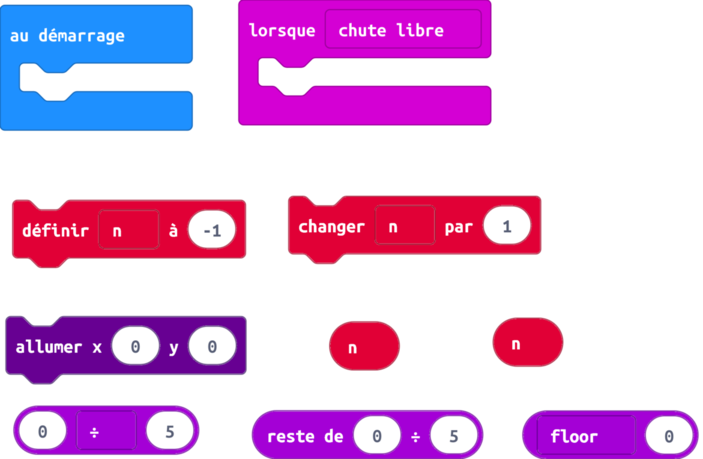
\includegraphics[width=0.6\textwidth]{res/mbChutesN1blocs.png}

\end{eleve}

\newpage
\subsubsection{Notes pour l'enseignant}

La difficulté de ce niveau tient dans l'affichage, ce qui pourrait facilement être contournée en affichant simplement un nombre plutôt qu'en allumant une nouvelle LED à chaque nouvelle chute. Néanmoins il est intéressant d'étudier comment ce problème d'affichage peut-être résolu simplement avec les deux opérateurs mathématiques arrondi et modulo.


\begin{minipage}[t]{0.6\linewidth}
    \begin{methode}~\\
        Pour résoudre ce problème, il suffit de programmer les instructions de la façon suivante :
        
        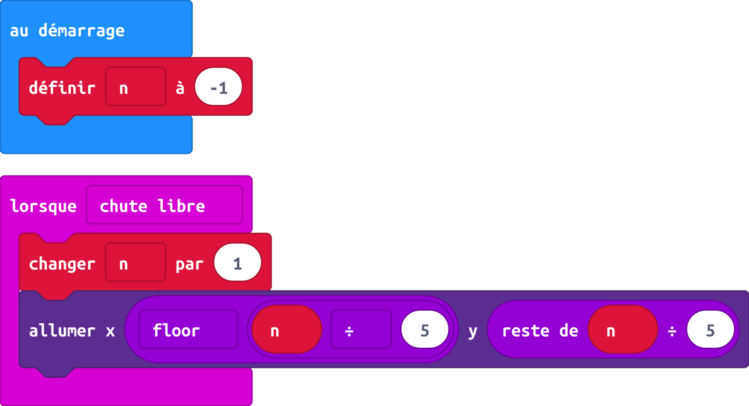
\includegraphics[width=\linewidth]{res/mbChutesN1proposition.png}
    \end{methode}
\end{minipage}
\hfill
\begin{minipage}[t]{0.4\linewidth}
    \begin{remarque}~\\
    La page vers l'interace de programmation avec le code prêt à télécharger :\\ \url{https://makecode.microbit.org/xxxxxxxxx}
    \end{remarque}
\end{minipage}

%
% activité de niveau 2
%
\newpage
\subsection{Niveau intermédiaire}
\subsubsection{Activité élève}

% commande perso \CARTOUCHE
%   5 paramètres : 
%       * durée
%       * public
%       * travail en maths
%       * travail en sciences
%       * travail en algo
\cartouche{1 h}{Term}{indicateurs statistiques}{mécanique}{affichage ; événement ; variable ; liste}

\begin{wrapfigure}{r}{2cm}
    
\includegraphics[width=\linewidth]{res/mbChutes.png}
\end{wrapfigure}
\begin{eleve}
Utilise \mb~pour déterminer une période moyenne \emph{une période moyenne d'oscillation} !

En t'aidant des blocs ci-dessous, programme \mb~pour : 
\begin{enumerate}
    \item programmer un événement lorsque l'appareil est en chute libre;
    \item itérer \emph{une variable} correspondant au \emph{nombre de chutes} subies par le \mb.
    \item utiliser le bloc \emph{temps d'exécution} pour mesurer la durée d'un nombre d'oscillation déterminé (10 par exemple)
    \item calculer la période moyenne d'oscillation (en ms et afficher le résultat
\end{enumerate}
Attention tous les blocs ne sont pas représentés : certains doivent être doublés et/ou modifiés.

\begin{center}
    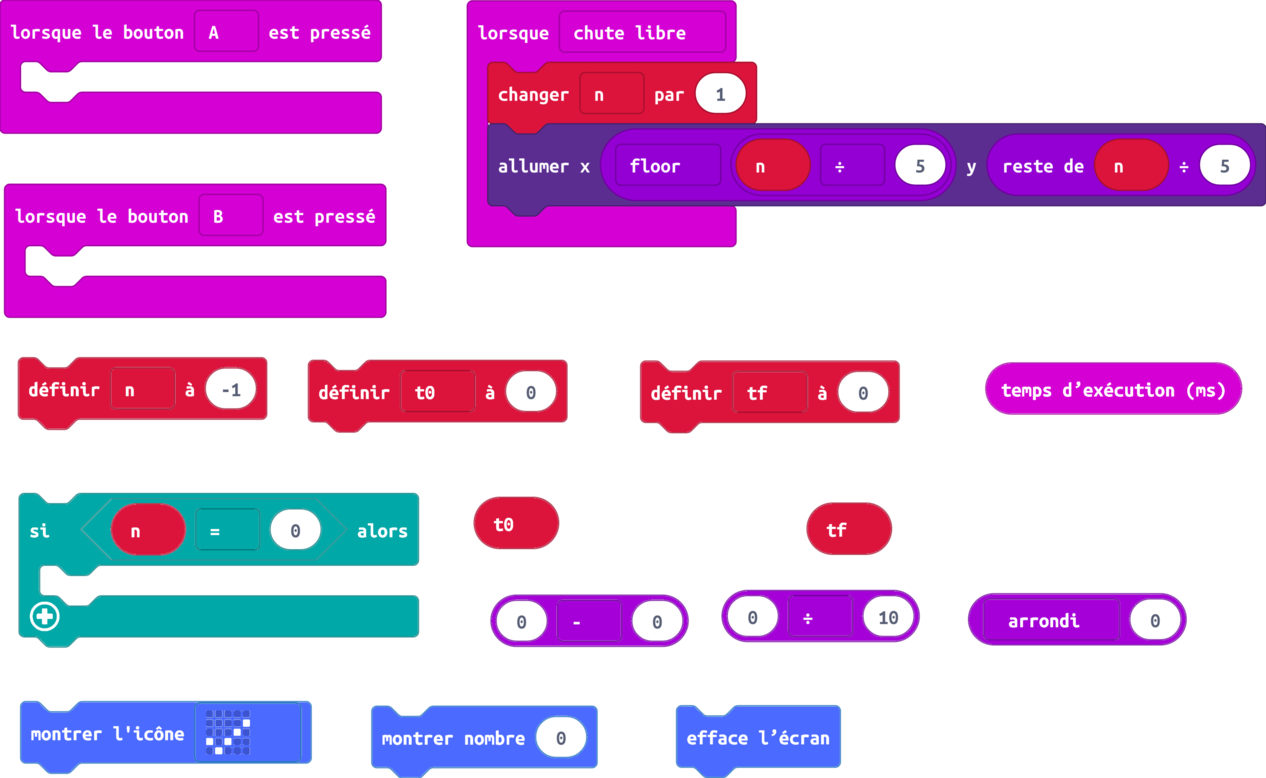
\includegraphics[width=0.65\textwidth]{res/mbChutesN2blocs.png}
\end{center}

\end{eleve}

\newpage
\subsubsection{Notes pour l'enseignant}



\begin{methode}
Pour résoudre ce problème, il suffit de programmer les instructions de la façon suivante :

\begin{center}
    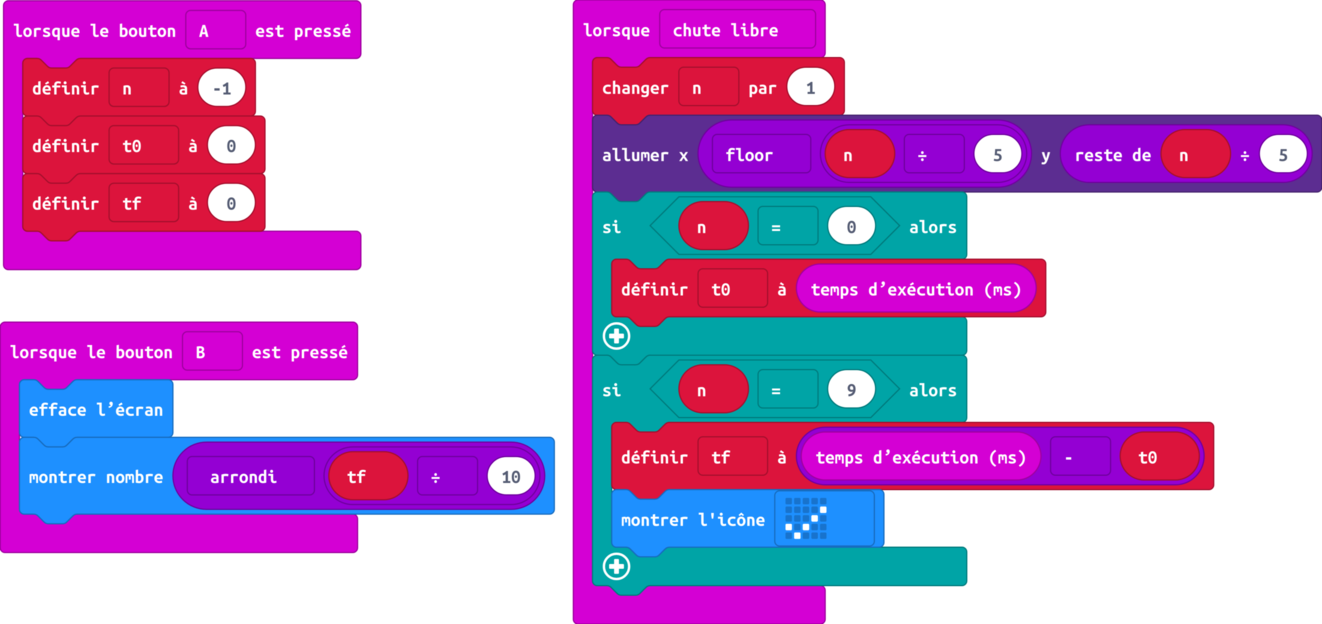
\includegraphics[width=0.95\linewidth]{res/mbChutesN2proposition.png}    
\end{center}

\end{methode}
